% !TEX encoding = UTF-8 Unicode
% $Header: /cvsroot/latex-beamer/latex-beamer/solutions/conference-talks/conference-ornate-20min.en.tex,v 1.6 2004/10/07 20:53:08 tantau Exp $

\documentclass[handout]{beamer}
\usepackage{icomma}
\usepackage{eurosym}

% This file is a solution template for:

% - Talk at a conference/colloquium.
% - Talk length is about 20min.
% - Style is ornate.

\mode<presentation>
{
  \usetheme{Warsaw}
  % or ...

  \setbeamercovered{transparent}
  % or whatever (possibly just delete it)
  
  \setbeamertemplate{navigation symbols}{}
  
  \newcommand*\oldmacro{}%
  \let\oldmacro\insertshorttitle%
  \renewcommand*\insertshorttitle{%
    \oldmacro\hfill%
    \insertframenumber\,/\,\inserttotalframenumber}
}

\usepackage[utf8]{inputenc}
% or whatever

\usepackage{times}
\usepackage{multirow}
\usepackage[T1]{fontenc}
\usepackage[french]{babel}
\usepackage{graphicx}
\usepackage{eso-pic}
\usepackage{color}
\usepackage{tikz}
\usepackage{wasysym}

% Or whatever. Note that the encoding and the font should match. If T1
% does not look nice, try deleting the line with the fontenc.

\title[]
{Mangaki.fr, système de recommandation\\de culture japonaise}

\author[]
{Ryan Lahfa \and Solène Pichereau \and Jill-Jênn Vie}

\institute[]
{Concours de la MCJP 2016}

\date
{15 janvier 2016}

\begin{document}

\definecolor{vert}{rgb}{0.07 0.54 0.07}

{
\setbeamertemplate{headline}[default]
\begin{frame}
	\titlepage
\end{frame}
}

\begin{frame}
	\frametitle{Japan Expo 2015}
	\begin{center}
	
\includegraphics[width=0.5\linewidth]{figures/japanexpo.png}\\
	\end{center}
	Mangas, anime, invités, concerts, cuisine, arts de vivre, ateliers pendant \alert{4 jours}
	\pause
	\begin{block}{Quelques chiffres}
	\begin{itemize}[<+->]
	\item 247\,473 visiteurs (72\,796 le samedi)
	\item 728 exposants dont 7 \% traditions, arts de vivre, littérature \& cuisine
	\item 550 heures de programmation
	\item 90~\% des visiteurs font des achats sur le festival
	\item 129~\euro{} de panier moyen
	\end{itemize}
	\end{block}
\end{frame}

\begin{frame}
	\frametitle{L'équipe Mangaki, une association de 18 membres}
	\begin{columns}
	\begin{column}{0.2\textwidth}
	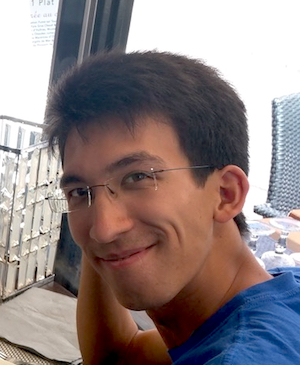
\includegraphics[width=\linewidth]{figures/jj.jpg}\\[-1mm]
	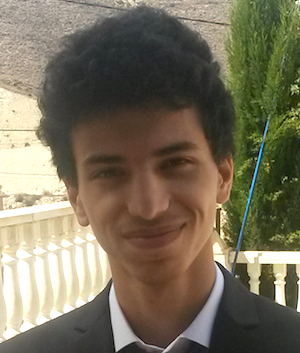
\includegraphics[width=\linewidth]{figures/ryan.jpg}\\[-1mm]
	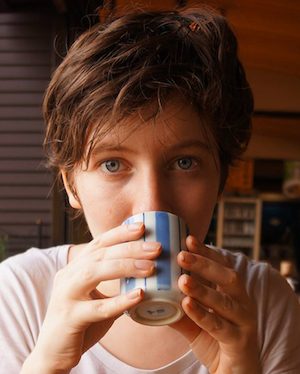
\includegraphics[width=\linewidth]{figures/solene.jpg}
	\end{column}
	\begin{column}{0.8\textwidth}
	\begin{block}{Jill-Jênn Vie, président}
	\begin{itemize}
	\item Doctorant en informatique à l'ENS Cachan
	\item Passionné de concours d'algorithmique
	\end{itemize}
	\end{block}
	\pause
	\begin{block}{Ryan Lahfa, développeur}
	\begin{itemize}
	\item Développeur freelance à Gigster
	\item Étudiant
	\end{itemize}
	\end{block}
	\pause
	\begin{block}{Solène Pichereau, directrice artistique}
	\begin{itemize}
	\item Graphiste manga à Delcourt
	\item Illustratrice pour Doujin Style
	\end{itemize}
	\end{block}
	\end{column}
	\end{columns}
\end{frame}

\begin{frame}
	\frametitle{Un système de recommandation}
	\centering
	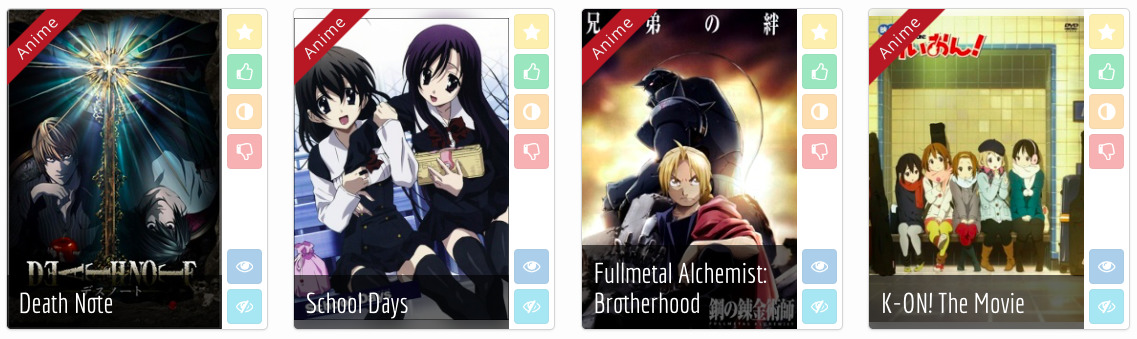
\includegraphics[width=0.9\linewidth]{figures/decks.jpg}
	\begin{block}{Principe}
	\begin{itemize}
	\item Un utilisateur s'inscrit et rentre ses préférences
	\item Mangaki lui recommande des mangas, anime, films susceptibles de lui plaire
	\end{itemize}
	\end{block}
	\pause
	\begin{block}{Objectifs}
	\begin{itemize}
	\item Elles doivent être \alert{pertinentes} (sinon l'utilisateur s'en va)
	\item \alert{Rapides} à calculer (sinon l'utilisateur s'en va)
	\end{itemize}
	\end{block}
\end{frame}

\begin{frame}
	\frametitle{Adaptable à d'autres bases de données}
	\begin{itemize}
	\item Romans japonais, films, musiques, jeux vidéo
	\item Le système peut faire de la \alert{recommandation croisée} : recommander des romans en fonction des mangas aimés.
	\item Certains anime recèlent d'autres facettes de la culture japonaise :
		\begin{itemize}
			\item \emph{Miss Hokusai}
			\item kend\=o, via \emph{Kurogane}
			\item hanafuda, via \emph{Summer Wars}
			\item karuta, via \emph{Chihayafuru}
		\end{itemize}
	\end{itemize}
\end{frame}

\begin{frame}
	\frametitle{Filtrage collaboratif}
	\begin{block}{Problème}
		\begin{itemize}
		\item On dispose de 1\,800 utilisateurs et 14\,000 œuvres à noter
		\item Chacun attribue une note à une \alert{partie} des items
		\item Base de données remplie à 1 \% (265\,000 notes)
		\end{itemize}
		$\Rightarrow$ Quels nouveaux items recommander à chaque utilisateur ?
	\end{block}
	\pause
	\begin{exampleblock}{Solution : les plus proches voisins}
		\begin{itemize}[<+->]
		\item On calcule un score de similarité entre utilisateurs
		\item On détermine les 20 utilisateurs les plus proches de vous
		\item On vous recommande ce qu'ils ont aimé
		\end{itemize}
	\end{exampleblock}
\end{frame}

\def\R{\mathcal{R}}
\def\N{N}

%\begin{frame}
%	\frametitle{Similarité}
%	Les points communs augmentent le score.
%	\begin{exampleblock}{Exemple}
%	\begin{center}
%	\begin{tabular}{cccccc}
%	& \emph{Paprika} & \emph{Oldboy} & \emph{Gattaca} & \emph{12 Monkeys}\\
%	Alice & 1 & -1 & 0 & 0\\
%	Bob & 1 & 1 & -1 & 0\\
%	Charles & 1 & -1 & 1 & -1
%	\end{tabular}\\
%	\vspace{5mm}
%	$score(Alice, Bob) = 1 + (-1) = 0$\\
%%	$score(Bob, Charles) = 1 + (-1) + (-1) = -1$\\
%	$score(Alice, Charles) = 1 + 1 = 2$\\
%	Alice est \alert{plus proche} de Charles que de Bob.
%	\end{center}
%	\end{exampleblock}
%\end{frame}

\begin{frame}
	\frametitle{Le problème du démarrage à froid}
	Les recommandations sont \alert{meilleures} si vous avez noté \alert{beaucoup} de films.
	\vspace{1cm}
	\pause
	\begin{itemize}
	\item Que faire au tout début ?
	\item Comment vous fournir des recommandations pertinentes tout en vous sollicitant le moins possible ?
	\end{itemize}
\end{frame}

\begin{frame}
	\frametitle{Mon sujet de thèse : les tests adaptatifs}
	Interview : \og \emph{Avez-vous aimé [ce film]} ? \fg\\
	En fonction de votre réponse, on choisit la question suivante.\vspace{1cm}

	\pause	
	Quelles œuvres choisir pour avoir une idée précise de vos goûts ?
	\pause
	\begin{itemize}[<+->]
	\item \alert{populaires}, pour que vous puissiez les noter
	\item \alert{controversés}, pour que ce soit informatif
	\end{itemize}
	\pause
\end{frame}

\begin{frame}
	\frametitle{Merci de votre attention !}
	\centering
	
\includegraphics{figures/mangaki.png}\raisebox{1em}{\Huge .fr}\\[8.4mm]
	\LARGE Jill-Jênn Vie\\[4.2mm]
	\raisebox{-3.5mm}{
\includegraphics[width=1cm]{figures/twitter.png}}\texttt{@mangakifr} \hfill \texttt{jjv@lri.fr}
\end{frame}

\end{document}